\section{Architettura}
L'architettura del prodotto è suddivisa tra Client e Server, inoltre si utilizzano le \glossario{API Rest} messe a disposizione dall'azienda Imola Informatica.
\subsection{Diagramma delle classi}
	\begin{figure}[H]
	\centering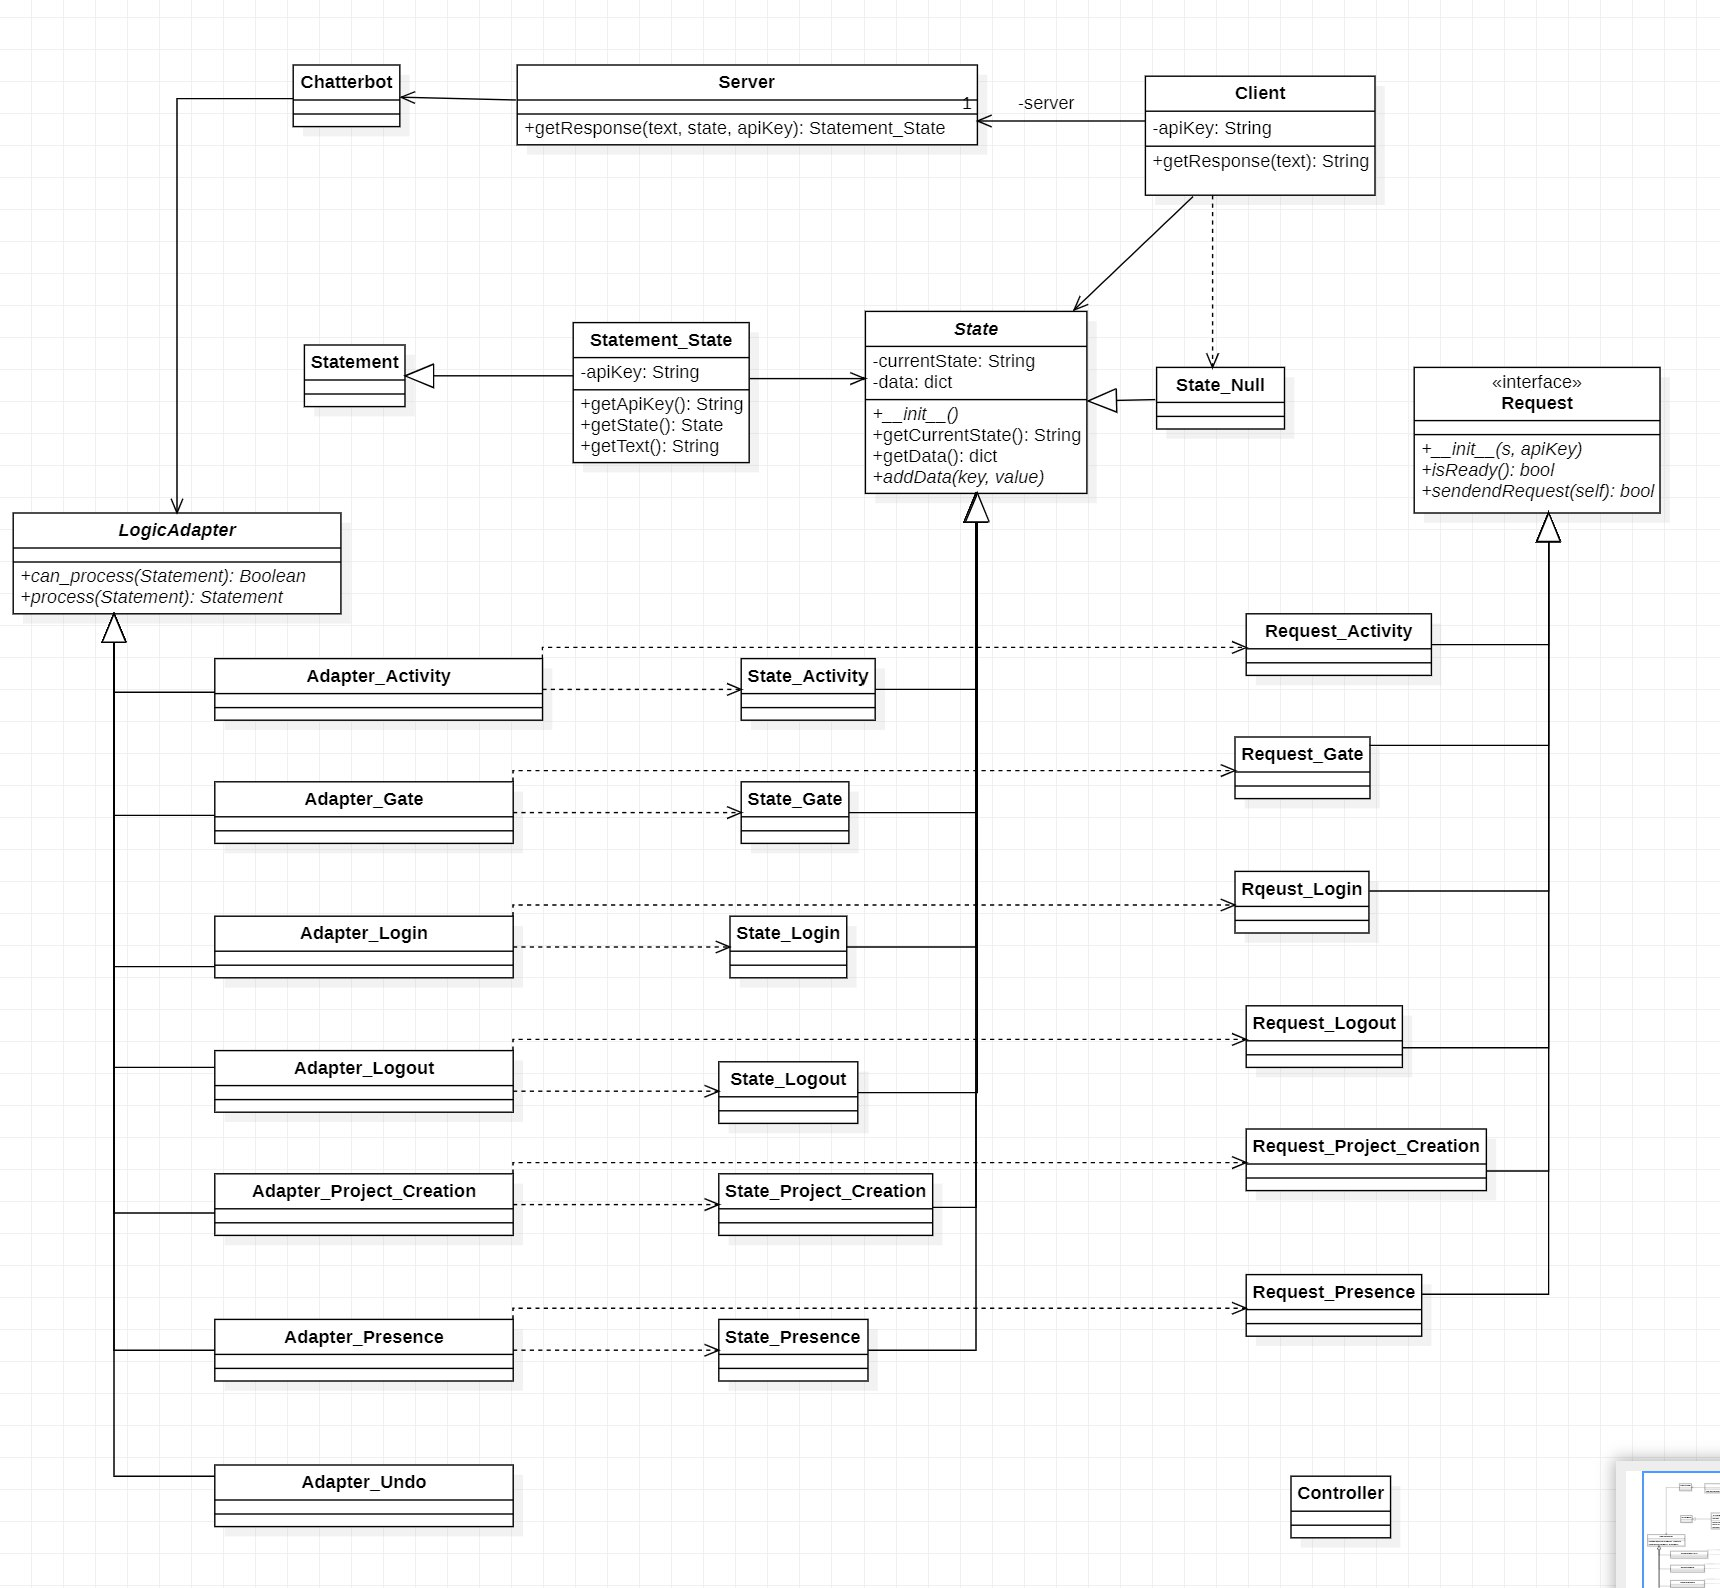
\includegraphics[scale=0.80]{images/diagramma_classi.jpg}
    \caption{Diagramma UML delle classi}
	\end{figure}
\subsection{App} Classe in cui vengono gestiti gli utenti e si interfaccia direttamente con l'utente.
\subsection{Client}
\subsection{Server}
\subsubsection{Chatterbot} Classe della libreria esterna scritta in \glossario{Python}. La classe \textit{Chatterbot} e le seguenti \textit{Statement}, \textit{Adapter} fanno parte della libreria.
\subsubsection{Statement} Classe fornita dalla libreria \glossario{Chatterbot} che rappresenta una singola entità, parola o frase che qualcuno può dire.
\subsubsection{LogicAdapter} Classe astratta fornita dalla libreria \glossario{Chatterbot} che permette al programmatore esterno di scrivere nuovi adapter. Dispone dei due metodi base di cui verrà fatto l'\glossario{overriding}:
    \begin{itemize}
        \item can\_process: metodo booleano che controlla tutte le varie condizioni e se tutto okay fa procedere il metodo \textit{process}.
        \item process: controlla ed elabora tutti i dati forniti così da produrre una risposta.
    \end{itemize}
\subsubsection{State} Interfaccia che definisce il contratto di tutti i vari stati e come dato privato si salva l'attuale stato corrente e pubblicamente dispone anche di un metodo per aggiungere informazioni necessarie per completare la richiesta in corso.
\paragraph*{State\_Null} Sottoclasse concreta di \textit{Stato} che simula uno stato nullo, utilizzato quando l'utente non ha effettuato nessuna richiesta.
\subsubsection{Statement\_State} Sottoclasse di Statement, cioè adatta l'adapter alla libreria chatterbot, in più ha lo stato attuale dell'utente, e l'api-key che dimostra l'autenticazione dell'utente che funge come input di ogni adapter.
\subsubsection{Request} Interfaccia che riceve i dati pronti verificandone la completezza e in base all'\textit{adapter} invia la richiesta \glossario{HTTP} alle \glossario{API Rest} di Imola per interagire con i loro servizi e soddisfare la richiesta dell'utente e infine ritorna ad adapter una risposta.
\subsubsection{Login} Classi \textit{Adapter\_Login}, \textit{State\_Login} permettono di effettuare il login
\subsubsection{Logout} Classe \textit{Adapter\_Logout} permette di effettuare il logout.
\subsubsection{Activity} Classi \textit{Adapter\_Activity}, \textit{State\_Activity} e \textit{Request\_Activity} per la funzionalità di consuntivare le ore dedicate ad un progetto compreso le eventuali ore di viaggio.
\subsubsection{Gate} Classi \textit{Adapter\_Gate}, \textit{State\_Gate} e \textit{Request\_Gate} per la funzionalità di apertura cancello
\subsubsection{Project\_Creation} Classi \textit{Adapter\_Project\_Creation}, \textit{State\_Project\_Creation} e \textit{Request\_Project\_Creation}
\subsubsection{Presence} Classi \textit{Adapter\_Presence}, \textit{State\_Presence} e \textit{Request\_Presence} per la funzionalità di registrazione della presenza
\subsubsection{Undo} Classe \textit{Adapter\_Undo} permette di annullare l'operazione in corso e di ricominciare la stessa o un'altra operazione dall'inizio.
\subsection{API Rest Imola Informatica} L'azienda ha fornito delle \glossario{API Rest} che permettono al \glossario{chatbot} di interagire con i loro sistemi aziendali. Sono facilmente consultabili a questo \href{https://apibot4me.imolinfo.it/}{\color{blue} link}.
%\newpage
%\begin{landscape}
	%\begin{figure}[H]
	%\centering\includegraphics[width=\linewidth]{images/diagramma_sequenza.jpg}
    %\caption{Diagramma di sequenza}
	%\end{figure}
%\end{landscape}
\newpage
